%%% Preamble
   \documentclass[11pt]{beamer}
   \usetheme{Boadilla}
   \useoutertheme{split}
   \useinnertheme{circles}
   \usepackage{fourier}
   \usefonttheme{structurebold}
   \usepackage{array}
   \usepackage[english]{babel}
   \usepackage{amsmath,amssymb}
   \usepackage[latin1]{inputenc}
   \usepackage{setspace}

   \usepackage{array}
   \usepackage{threeparttable}
   \usepackage{colortbl}
   \usepackage{multirow}
   \usepackage{amsthm}
   \usepackage{float,graphicx,color}
   \newtheorem*{thm}{Theorem}
   \theoremstyle{definition}
   \newtheorem*{defn}{Definition}
   \newcommand\boldline{\arrayrulewidth{1pt}\hline}
   \newcommand\ve{\varepsilon}
   \providecommand{\norm}[1]{\lVert#1\rVert}


   \setbeamercovered{dynamic}

   \title[Crystal Radio]{Germanium Diode Crystal Radio}
   \author[Honick and Lyon]{\textbf{Chuck Honick} \and \textbf{Spencer Lyon}}
   \date{\today}


\begin{document}
      \frame{\titlepage}

      \section{Intro}

         \begin{frame}
                  \frametitle{Some facts}
                  \begin{itemize}
                        \item First used to receive Morse code signals
                        \vspace{3mm}
                        \item Have since been to pick up vocal broadcasting signals
                        \vspace{3mm}
                        \item  No battery power; all energy is from radio waves received by antenna
                        \vspace{3mm}
                        \item Reliable and cheap $\rightarrow$ popular
                        \vspace{3mm}
                        \item No amplification = weak (quiet) signal
                  \end{itemize}
         \end{frame}


         \begin{frame}
                  \frametitle{How it works}
                  \begin{itemize}
                        \item 3 main parts
                        \vspace{2mm}
                        \begin{enumerate}
                           \item Antenna
                           \vspace{2mm}
                           \item Tuning circuit
                           \vspace{2mm}
                           \item Semiconductor crystal detector
                        \end{enumerate}
                        \vspace{2mm}
                        \item Also, to hear the signal you need a speaker or earpiece
                  \end{itemize}
         \end{frame}

      \section{Method}

         \subsection{Antenna}
               \begin{frame}
                     \frametitle{Antenna Theory}
                     \begin{itemize}[<+->]
                           \item Converts energy in electromagnetic radio waves to AC current
                           \vspace{1.5mm}
                           \item For best performance, antenna length should be $\frac{1}{4}$ of signal wavelength
                           \vspace{1.5mm}
                           \begin{itemize}
                              \item common AM radio frequency ($f$) range is $(531-1611) kHz$
                              \vspace{1mm}
                              \item wavelength: $\lambda = \frac{c}{f} = \frac{3 \times 10^8 m/sec}{f Hz} \rightarrow$ range $(186-564) m$
                              \vspace{1mm}
                              \item Ideal antenna length $l = \lambda/4 = (46-141) m$
                              \vspace{1mm}
                           \end{itemize}
                           \vspace{1.5mm}
                           \item Antenna is only "power source" in the circuit
                           \vspace{1.5mm}
                           \item Larger antenna results in more power (louder signal)
                     \end{itemize}
               \end{frame}

               \begin{frame}
                  \frametitle{Our antenna}
                  \begin{itemize}
                        \item We tried two different antennas
                            \vspace{2mm}
                        \begin{enumerate}
                            \item 25 ft (7.62 m) of aluminum single strand insulated wire
                            \vspace{1.5mm}
                            \item 72 ft (21.95 m) of copper single strand insulated wire
                        \end{enumerate}
                        \vspace{2mm}
                        \item Recall that optimal antenna length is between 46-141 m
                        \vspace{2mm}
                        \item Copper wire did much better than the aluminum
                  \end{itemize}
                \end{frame}

            \subsection{Tuner}
                \begin{frame}
                  \frametitle{Tuning circuit theory}
                  \begin{itemize}[<+->]
                        \item Consists of an inductor (L) and a capacitor (C)
                        \vspace{2mm}
                        \item Current flows between the capacitor and the solenoid
                        \vspace{2mm}
                        \item Works a lot like a tuning fork (resonance)
                        \vspace{2mm}
                        \item The received signal frequency matches the resonant frequency of the LC circuit ($f = \frac{1}{2 \pi \sqrt{LC}}$)
                        \vspace{2mm}
                        \item Different "loops" on the solenoid allow the user to change inductance ($L = \frac{\mu N^2 A}{l}$) and therefore change resonant frequency
                  \end{itemize}
                \end{frame}

                \begin{frame}
                  \frametitle{Our tuning circuit}
                  \begin{itemize}
                        \item To build the tuning circuit, we followed this circuit diagram
                        \includegraphics[height=1.5in, width=3in]{Figures/circuitDiagram}
                        \item Our solenoid has 60 turns ($N$ = 60)
                        \item Capacitor value: 0.001 $\mu F$
                        \item Resistor value: 82 $k\Omega$
                  \end{itemize}
                \end{frame}

            \subsection{Detector}
                  \begin{frame}
                  \frametitle{Semiconductor crystal detector}
                  \begin{itemize}[<+->]
                        \item Rectifies the AM frequency leaving only positive frequency components
                        \vspace{2mm}
                        \item This frequency is is then filtered with a resistor and capacitor and fed to audio device
                        \vspace{2mm}
                        \item Old crystal radios used Galena (lead sulfide), but that isn't the most efficient
                        \vspace{2mm}
                        \item Germanium diodes are optimal because a low forward voltage drop makes them more sensitive
                        \vspace{2mm}
                        \item We used a NTE109 Germanium diode (fast-switching)
                  \end{itemize}
            \end{frame}


            \begin{frame}
            \frametitle{Audio output}
                \begin{itemize}
                    \item We initially tried headphones, but they didn't work
                    \vspace{1mm}
                    \begin{itemize}
                        \item Input impedance was too low
                        \vspace{1.5mm}
                        \item No signal or sound amplification
                    \end{itemize}
                    \vspace{2mm}
                    \item We then used externally powered speakers
                    \vspace{1mm}
                    \begin{itemize}
                        \item  Much better because impedance was very high
                        \vspace{1.5mm}
                        \item External power amplified the sound signal
                    \end{itemize}
                \end{itemize}
            \end{frame}


      \section{Results}
         \begin{frame}
              \frametitle{The Final Product}
              \centering
              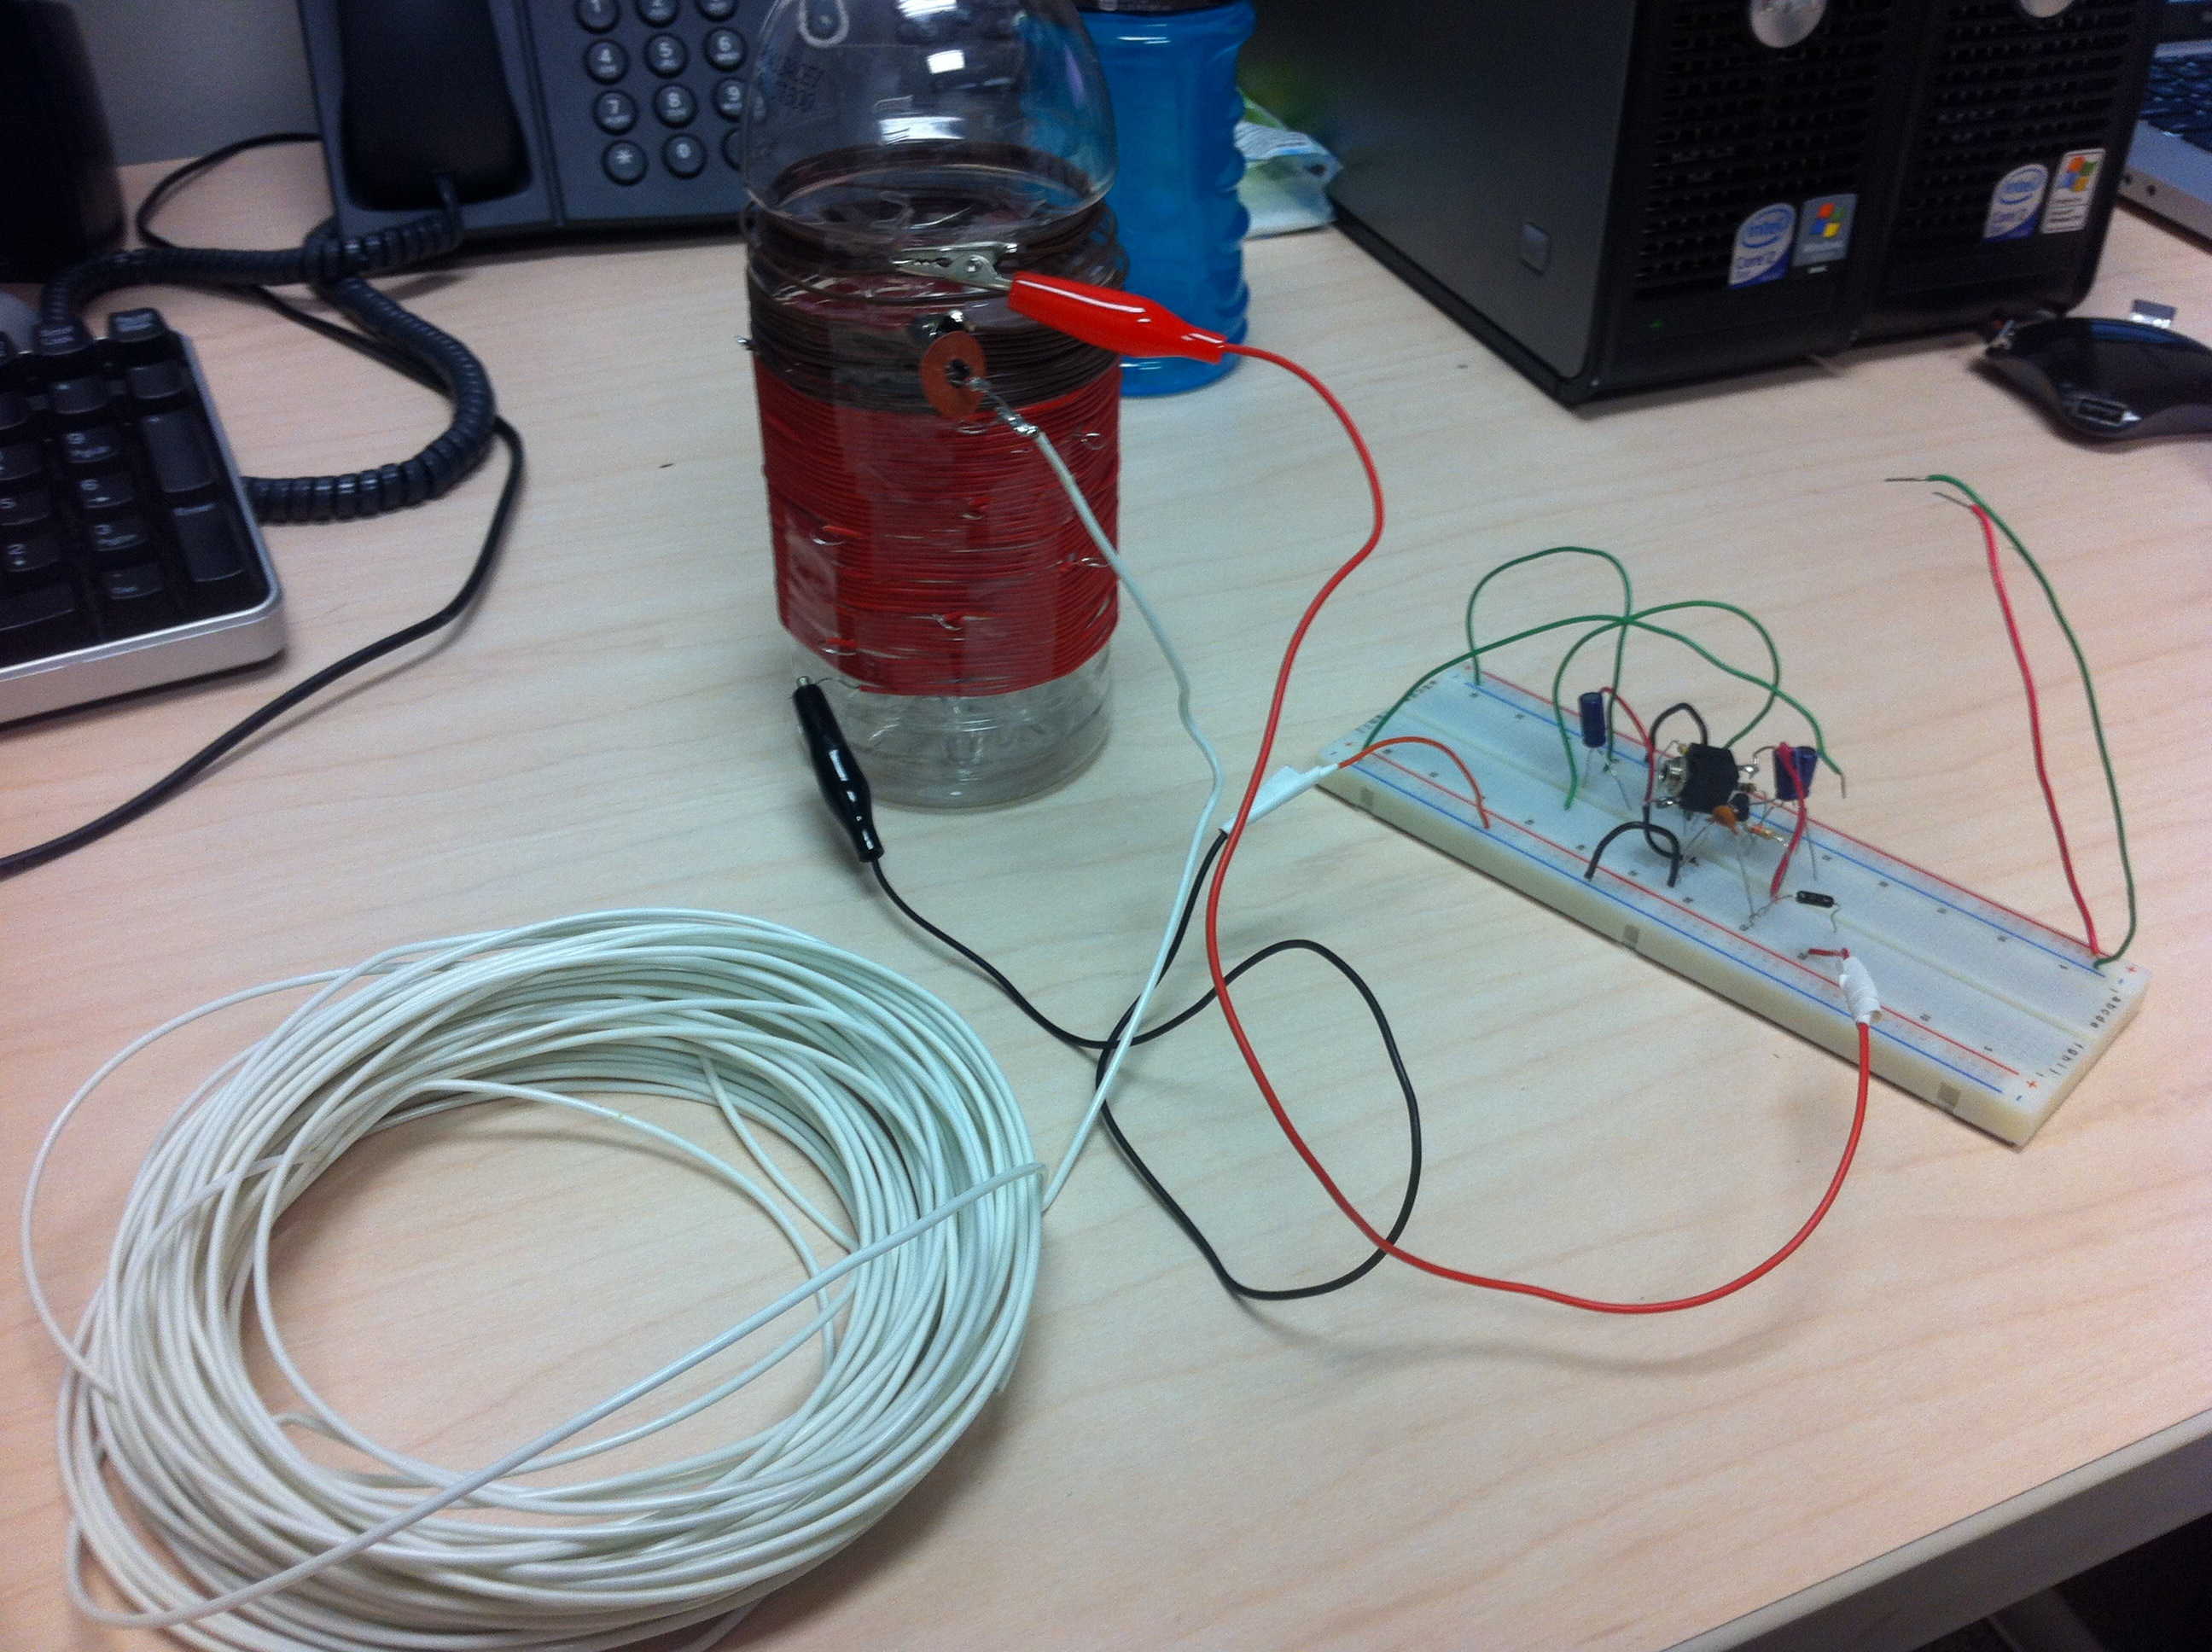
\includegraphics[height=2.5in, width=4.3in]{Figures/everything.jpeg}
         \end{frame}

         \begin{frame}
              \frametitle{Demo}
              \begin{itemize}
                  \item Tune in to 1280 The Zone!
              \end{itemize}
         \end{frame}

         \section{Interpretation and Conclusion}
         \begin{frame}
              \frametitle{Interpretation}
               \begin{itemize}
                     \item There are many ways we could improve our radio
                     \vspace{2mm}
                     \begin{itemize}[<+->]
                          \item Tune the antenna with capacitor which increases the signal/noise ratio
                          \vspace{1mm}
                          \item We have single capacitor for filter, using a variable capacitor would allow us to pick up different frequencies
                          \vspace{1mm}
                          \item Include a signal (or audio) amplifier to make signal to the audio device stronger
                          \vspace{1mm}
                          \item Build a larger solenoid and/or use longer antenna
                     \end{itemize}
               \end{itemize}
         \end{frame}

\end{document}
